%%%%%%%%%%%%%%%%%%%%%%%%%%%%%%%%%%%%%%%%%%%%%%%%%%%%%%%%%%%%%%%%%%%%%%
% UMB-CS110-2015S: Introduction to Computing
% Copyright 2015 Pejman Ghorbanzade <pejman@ghorbanzade.com>
% Creative Commons Attribution-ShareAlike 4.0 International License
% More info: https://github.com/ghorbanzade/UMB-CS110-2015S
%%%%%%%%%%%%%%%%%%%%%%%%%%%%%%%%%%%%%%%%%%%%%%%%%%%%%%%%%%%%%%%%%%%%%%

\def \topDirectory {.}
\def \texDirectory {\topDirectory/src/main/tex}

\documentclass[12pt,letterpaper,twoside]{article}
\usepackage{\texDirectory/template/style/directives}
\usepackage{\texDirectory/template/style/assignment}
%%%%%%%%%%%%%%%%%%%%%%%%%%%%%%%%%%%%%%%%%%%%%%%%%%%%%%%%%%%%%%%%%%%%%%%%%%%%%%
% CS110: Introduction to Computing
% Copyright 2015 Pejman Ghorbanzade <mail@ghorbanzade.com>
% Creative Commons Attribution-ShareAlike 4.0 International License
% https://github.com/ghorbanzade/UMB-CS110-2015S/blob/master/LICENSE
%%%%%%%%%%%%%%%%%%%%%%%%%%%%%%%%%%%%%%%%%%%%%%%%%%%%%%%%%%%%%%%%%%%%%%%%%%%%%%

\course{id}{CS110}
\course{name}{Introduction to Computing}
\course{venue}{Tue/Thu, 5:30 PM - 6:45 PM}
\course{semester}{Spring 2015}
\course{department}{Department of Computer Science}
\course{university}{University of Massachusetts Boston}

\instructor{name}{Pejman Ghorbanzade}
\instructor{title}{}
\instructor{position}{Student Instructor}
\instructor{email}{pejman@cs.umb.edu}
\instructor{phone}{617-287-6419}
\instructor{office}{S-3-124B}
\instructor{office-hours}{Tue/Thu 19:00-20:30}
\instructor{address}{University of Massachusetts Boston, 100 Morrissey Blvd., Boston, MA}


\begin{document}

\doc{title}{Assignment 4}
\doc{date-pub}{Apr 06, 2015 at 00:00 AM}
\doc{date-due}{Apr 16, 2015 at 5:30 PM}
\doc{points}{8}

\prepare{header}

\section*{Question 1}

Back to Dalton Brothers! Develop a simple class \texttt{Brother.java} and its data memebrs and methods as you think best fits this program. Neglecting their original heights, write a program \texttt{Daltons3.java} that uses the \texttt{Brother.java} class to sort Joe, William, Jack and Averell after getting their heights from the user. The program should output names of the brothers in ascending order of their heights as specified.

\begin{figure}[H]\centering
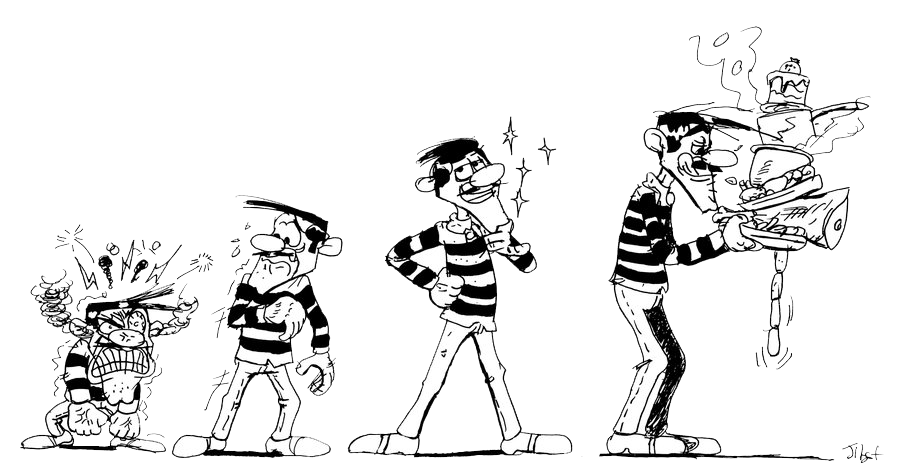
\includegraphics{\texDirectory/template/images/daltons.png}
\end{figure}

\section*{Question 2}

A student recently found a scrap of paper in MBTA Red line train on which the following code was written. Without modifying the code, develop a class \texttt{Elevator.java} to be used by this program.
\lstset{language=java}
\begin{lstlisting}
public class ElevatorTest {
	public static void main(String[] args) {
		Elevator.currentLevel(); //outputs current floor
		Elevator.go(2); //moves the elevator two floors up
		Elevator.currentLevel();
	}
}
\end{lstlisting}

\section*{Question 3}

Objective is to simulate a circle-shaped pond with 100 meters radius, in which there are initially 100 salmons and one shark. As sharks and salmons know swimming, they continually wander around the pond. It's all about survival! To avoid starving to death, the shark must eat. To avoid extinction, salmons reproduce. Contrary to what it seems however, the shark has a very poor fate. If it doesn't eat for too long it will sadly die. If it manages to eat all the salmons and there are no more to eat, it won't be able to escape his destiny either. It's not about survival then. It's all about time!
\begin{figure}[H]\centering
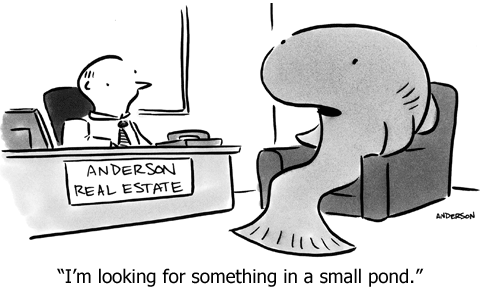
\includegraphics[width=8cm,height=5cm]{\texDirectory/template/images/pond.png}
\end{figure}

Write a program \texttt{Simulation.java} that determines how many days the shark will live. Develop classes \texttt{Fish.java}, \texttt{Salmon.java}, \texttt{Shark.java} and \texttt{Pond.java} with their class members as you think best fits this program. Use the following assumptions.
\begin{itemize}[itemsep=1mm] \parskip=0pt \parsep=0pt
\item[] Fish are initially positioned randomly in the pond.
\item[] Fish move randomly in the pond.
\item[] Salmons move 10 meter per hour.
\item[] Salmons reproduce every day.
\item[] Salmons don't age and don't need to eat.
\item[] Salmons won't die unless they are eaten.
\item[] The shark moves 40 meters per hour in one direction.
\item[] The shark cannot eat while it's moving.
\item[] The shark is always hungry and never loses interest in eating.
\item[] The shark swallows all salmons within its 20 meters of proximity in a blink of an eye.
\item[] The shark dies if it does not eat in three days.
\item[] The shark is initially well fed.
\end{itemize}

\prepare{footer}

\end{document}
